% !TEX root = diss.tex

\chapter{Introduction}

\section{Background}

Radicals are chemical species that tend to be highly reactive due to the presence of one or more unpaired electrons. Living systems depend on radical processes as part of normal metabolism\cite{Halliwell2015} but biomaterials, such as proteins, are susceptible to radical-induced damage. Radical-induced oxidation of biomaterials has been implicated in a number of degenerative disease states, including cancer, Alzheimer's, Parkinson's, and multiple sclerosis.\cite{Barnham2004, Valko2007, Hwang2013, Halliwell2007}

In biological systems, radicals are derived from many sources. Exogenous sources include solar radiation and air pollutants, while endogenous sources include \emph{in vivo} transition metal-ion redox processes, such as the electron transport chain involved in cellular respiration.\cite{Turrens2003} Some processes in the electron transport chain may transfer an electron to molecular oxygen, forming the superoxide anion (\ch{O2^{.-}}). Superoxide is not a strong oxidant on its own, however it may become protonated to form the more reactive hydroperoxyl radical,\cite{Kozmer2014} or disproportionate spontaneously or catalytically through metalloenzymes such as superoxide dismutase, leading to the formation of highly reactive oxygen-centred radicals. Oxygen-centred radicals derive from reactions of \ch{O2} with redox-active metals.\cite{Halliwell2015}

Oxygen-centred radicals, known as reactive oxygen species (ROSs) in biology, are particularly important and common due to the previously described nature of aerobic respiration. The ROSs which are of primary concern are the highly reactive hydroxyl radicals (\ch{HO^.}), alkoxyl radicals (\ch{RO^.}), superoxide (\ch{HOO^.}/\ch{O2^{.-}}), and peroxyl radicals (\ch{ROO^.}).\cite{Halliwell2015} The oxidation of proteins by ROSs occurs through a radical chain mechanism which has been studied experimentally in detail.\cite{Berlett1997, Davies2016} This chain reaction occurs when an ROS initiates a radical chain reaction through hydrogen atom transfer (HAT), single electron transfer, or addition reactions with protein substrates, leading to rapid propagation and formation of new radicals. HAT is an extremely important reaction in the context of oxidative damage. The focus of my work is the development of an understanding of the fundamental chemistry involved in protein oxidation through studying small model systems.

Proteins are the most abundant biomaterial in most mammalian biological systems,\cite{Davies2005} thus understanding their degradation is essential to understanding degenerative disease. Because proteins are composed of as many as 20 common amino acid side-chains, as well as the common peptide backbone, there are a large number of possible reactions. Some of the reactions involved in protein oxidation are shown in~\ref{fig:proteinoxidation}.

\begin{scheme}[!htbp]
  \centering
  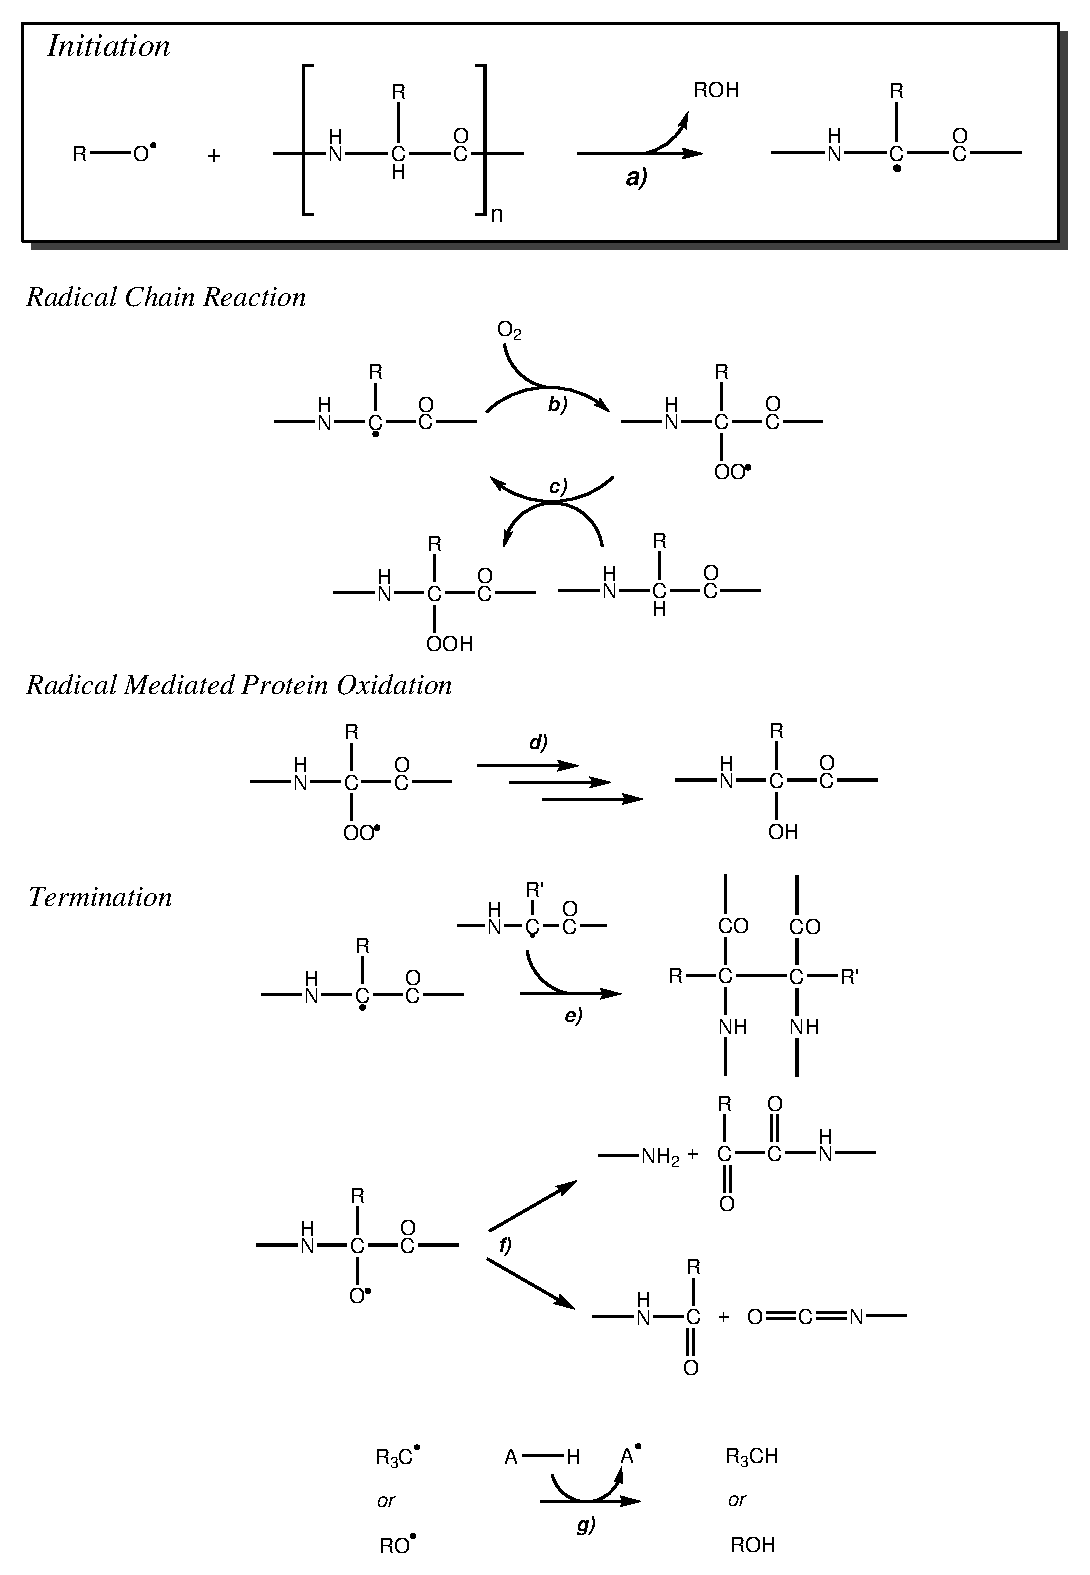
\includegraphics[height=12cm]{figures/proteinoxidation-2.eps}
\caption[Common reactions involved in the protein oxidation.]{Common reactions involved in the protein oxidation. The reactions are as follows: \textbf{a)} initiation of radical chain through abstraction by an oxygen centred radical to generate an $\alpha$-carbon-centred radical, \textbf{b)} radical addition of molecular oxygen, \textbf{c)} propagation of the radical chain reaction generating another $\alpha$-carbon radical and a peroxide. \textbf{d)} Radical mediated protein oxidation proceeds through multiple steps involving oxygen centred radicals and molecular oxygen result in the generation of a reduced amide (alcohol). Termination of the radical chain reaction can occur in several ways, including: \textbf{e)} cross-linking mechanism of two carbon-centred radicals, \textbf{f)} fragmentation pathways of an oxygen-centred radical intermediate, or \textbf{g)} HAT with an antioxidant (AH).}
\label{fig:proteinoxidation}
\end{scheme}

Initial abstraction (Reaction \textbf{a}) often occurs at the $\alpha$-carbon position (\ch{$\alpha$-CH}), forming a carbon-centred radical (\ch{$\alpha$-C^.}) which is partially delocalized in the $\pi$-system of the neighbouring amide and carbonyl groups. Studies have indicated that the stability of \ch{$\alpha$-C^.} is determined by stereo-electronic considerations related to the planarity of the amide group.\cite{Salamone2014b} As such, steric bulk in the side-chains, as well as local protein structure (helix, sheet, etc.) can constrain radical geometries. For example, the most stable $\alpha$-carbon radicals occur at glycine residues in antiparallel $\beta$-sheets, whereas other bulkier residues and secondary structures lead to loss of captodative stabilization.\cite{Rauk2000} Amino acid side-chains are also susceptible to oxidation. Those side-chains containing sulphur,\cite{Stadtman2004} as well as tyrosine (which has a fairly weak phenolic O-H bond of about 89 \kcalmol),\cite{Mulder2005} are particularly susceptible to oxidation.

Propagation of the radical chain reaction occurs through various processes. In the presence of molecular oxygen, rapid addition occurs at the newly formed \ch{$\alpha$-C^.} (Reaction \textbf{b}), generating a peroxyl radical, which can carry forward through further HAT reactions (Reaction \textbf{c}).\cite{Stadtman2003} The mechanism involved in the radical mediated oxidation of proteins has been studied experimentally using techniques involving ionizing radiation.\cite{Garrison1962,Garrison1987} The course of this process is complexly dependent on the availability of either singlet oxygen (\ch{^1O2}), or superoxide (\ch{O2^{.-}}) or the protonated form, peroxyl radical (\ch{^.OOH}). A detailed analysis of this process is outside the scope of this thesis, but ultimately, these reactions lead to the generation of a hydroxyl-amide (Reaction \textbf{d}).

The radical chain reaction can be terminated through several mechanisms, including protein-protein cross-linking (Reaction \textbf{e}), or protein fragmentation (Reaction \textbf{f}). Reactions with antioxidants (\ch{A-H}, Reaction \textbf{g}) also terminate the chain reaction by removing the radical from the protein system. The sum total of all these processes contribute to the accumulation of oxidized proteins which are associated with many degenerative diseases.\cite{Halliwell2006} HAT reactions which are important steps in the initiation, propagation, and termination reactions of protein oxidation are investigated through small molecular models in this thesis.

\section{Details of HAT reactions}

Developing an understanding of protein and other biomolecular oxidation requires an understanding of the deceptively simple HAT reactions involved. Formal HAT reactions are a fundamental radical chemical transformation that have been studied for more than a century.\cite{Kochi1973, Parsons2000} From an experimental perspective, HAT reactions which involve oxygen-centred radicals and non-radical organic substrates are reasonably well characterized: the effects of different solvents are well understood.\cite{Litwinienko2007} However, the main challenge faced by many experiments is elucidating the mechanistic details of a reaction. This is a problem that can be examined by quantum chemistry, which is the approach that I shall take. Background on the theory used in this thesis is given in Chapter~\ref{ch:theory}.

In order to investigate HAT reactions, we need to consider the mechanism in detail. For a simple HAT reaction, there exists several possible mechanisms by which this transformation can occur. The two most common concerted mechanisms are direct HAT and proton-coupled electron transfer (PCET). At the basic level, direct HAT involves the transfer of an electron and proton through the same set of acceptor/donor orbitals, while PCET involves the transfer of an electron and proton through different sets of orbitals. In practise, this distinction is poorly described, and is still an active topic of discussion in the literature.\cite{Cukier1998, Mayer2002, Stubbe2003, Mayer2004, DiLabio2007, Huynh2007, HammesSchiffer2008, Mayer2010, Weinberg2012, HammesSchiffer2015, MunozRugeles2017}

The prototypical example demonstrating the difference between direct HAT to PCET comes from the work of Mayer et al.,\cite{Mayer2002} that describes the self-exchange reactions of benzyl-toluene and phenoxyl-phenol, shown in~\ref{fig:self1}. In their work, the transition state (TS) structures were obtained through theoretical studies. These complexes are oriented so that the aromatic rings are trans relative to one another. In this geometry, the benzyl-toluene pair undergoes direct HAT, with the $2p-\pi$ orbital of the benzylic carbon radical oriented at the benzylic hydrogen on toluene. This is described as direct HAT, as the orbital containing the radical overlaps with the C-H $\sigma^*$ anti-bonding orbital, and thus the transfer of the H atom occurs through the same set of orbitals (see~\ref{fig:self1} A).

\begin{scheme}[htb]
\vspace{1cm}
\begin{overpic}[width=0.85\textwidth]{figures/PhCH3-PhCH2.eps}
  \put(-10,35) {\large\textbf{A.}}
\end{overpic}
\begin{overpic}[width=0.85\textwidth]{figures/PhOH-PhO.eps}
  \put(-10,15) {\large\textbf{B.}}
\end{overpic}
\caption{Self-exchange reactions of the \textbf{A.} benzyl-toluene couple through direct HAT \textbf{B.} phenoxyl-phenol couple through PCET.}
\label{fig:self1}
\end{scheme}

For the phenoxyl-phenol pair (see~\ref{fig:self1} B), a fairly strongly hydrogen bonded pre-reaction complex is first formed with a predicted gas-phase binding enthalpy $\Delta H$ of -8.1 \kcalmol. As a result of this strong interaction, the TS structure is such that the phenoxyl radical nominally occupies an oxygen $2p$ orbital that is perpendicular to the hydrogen bond. Therefore, in order to undergo direct HAT, the hydrogen bond between the OH and O lone pair must break, and a new, weaker hydrogen bond with the nominally O-centred radical must form. Alternatively, the hydrogen bonded pre-reaction complex geometry allows the orbital containing the radical to overlap with the $2p$ lone pair of the phenol moiety, and the conjugated aromatic $\pi$-systems in the TS complex. This overlaps results in a TS complex with a singly occupied molecular orbital (SOMO) that is of $\pi$-symmetry and highly delocalized. Accordingly, the proton is transferred through the hydrogen bond and the electron is transferred through the $\pi$-system. This reaction has an enthalpic barrier height ($\Delta H^{\ddagger}$) of 5.0 \kcalmol~ relative to the hydrogen bonded complex, so that the barrier is 3.1 \kcalmol~ below the separated reactants.

The work by \citet{Mayer2002} suggests that hydrogen bonding is a necessary, but not sufficient, condition for PCET to occur. This then implies that PCET is not possible between molecules which do not possess hydrogen bonding moieties, such as carbon atoms. Work by other authors has shown this to be untrue.\cite{Hatcher2007, DiLabio2007} In particular, \citet{DiLabio2007} demonstrated that \citet{Mayer2002} neglected the important contributions of $\pi-\pi$ interactions and lone pair-$\pi$ interactions. Computational studies revealed the existence of a TS structure for the benzyl-toluene couple which is 3.7 \kcalmol~ lower in energy than previously reported. This structure orients the aromatic rings in an optimal ``parallel-displaced'' conformation, as observed in the benzene-benzene non-covalently bound dimer.\cite{Sinnokrot2002}
Analysis of the TS structure highest-occupied molecular orbital (HOMO) reveals bonding character between the two $\pi$-systems, while the SOMO shows anti-bonding character between the $\pi$-systems, as well as both C-H bonds. Thus, there exists a net partial bonding interaction between the two $\pi$-systems, opening up an additional electronic channel for electron transfer to occur, while the hydrogen bond allows for proton transfer. DiLabio and Johnson also suggested that the phenol-phenoxyl couple likely prefers a $\pi$-stacked TS structure, and compare this to a structural analogue, a naturally occurring tyrosyl-tyrosine couple, which they demonstrated proceeds through a PCET mechanism. Other authors have confirmed the existence of a $\pi$-stacked TS structure for the phenol-phenoxyl couple.\cite{Sirjoosingh2011, HammesSchiffer2015, MunozRugeles2017} In the work of \citet{MunozRugeles2017}, it was demonstrated that the preference for $\pi$-$\pi$ stacking vs. non-stacking cannot be used as a general criteria for differentiating between the PCET and HAT mechanisms. Interestingly, they also showed that reaction barrier heights for the PCET mechanism are systematically lower than those for direct HAT mechanism.

HAT can also occur through a PCET mechanism for species which have lone pair-$\pi$ or lone pair-lone pair overlap in the TS complex.\cite{DiLabio2007, DiLabio2005} \citet{DiLabio2007} showed that the formal HAT reaction between phenol and the $t$-butyl peroxyl radical exhibits orbital overlap between the non-radical O-lone pair of $t$-butyl peroxyl and the aromatic $\pi$-system of phenol in the lowest energy cisoid TS complex. As with the benzyl-toluene couple, there is both a bonding interaction in the HOMO of the TS structure, and an anti-bonding interaction in the SOMO of the TS structure. Therefore, there exists a net partial bonding interaction which allows electron transfer through the lone pair-$\pi$ interaction and proton transfer through the hydrogen bond. \citet{DiLabio2005} also showed that iminoxyl-oxime self-exchange reactions occur through a five-centred PCET TS complex. The lowest energy transition states for iminoxyl-oxime couples are cisoid, such that the lone pairs of the nitrogen centres overlap, opening a channel for electron transfer, while proton transfer occurs between the two oxygen centres.

Bearing in mind there is not an obvious way to explore the related differences in mechanism experimentally, computational examination of formal HAT reactions enables analysis of the mechanism of these reactions. Herein, I shall consider the existence of these mechanisms on a continuum: Reactions where an unambiguous $\pi$-$\pi$ stacked PCET TS structure is formed (for example the \ch{PhO^. + PhOH} self-exchange reaction) have the most PCET character, and therefore have the lowest reaction barriers; while reactions with an unambiguous direct HAT TS structure is formed (for example the \ch{CH3^. + CH4} self-exchange reaction) have the most HAT character, and therefore have the highest reaction barriers. In the middle are PCET reactions which may occur through either LP-$\pi$ (more PCET character) or LP-LP interactions (less PCET character). In doing so, important insight is gained from understanding the electronic behaviour of these reactions. In this vein, the investigation of the physico-chemical nature of HAT reactions shall be the central theme of this thesis.

Consider for a moment the potential energy surface (PES) for an arbitrary chemical reaction, which is a complex hypersurface that depends on many variables. Theoretical methods can be used to generate a full PES, however, this quickly becomes computationally infeasible as the number of atoms in a system increases. Typically this problem can be simplified by examining only the relevant degrees of freedom. Often, the two most important coordinates can be isolated, giving a three-dimensional PES.\@ Furthermore, in chemistry we often simplify this problem to two-dimensions using the so-called intrinsic reaction coordinate, which is the lowest energy cross section of a higher dimension PES.\@ This yields a reaction coordinate diagram, as is illustrated below in~\ref{fig:pes}.

\begin{figure}[htb]
  \centering
  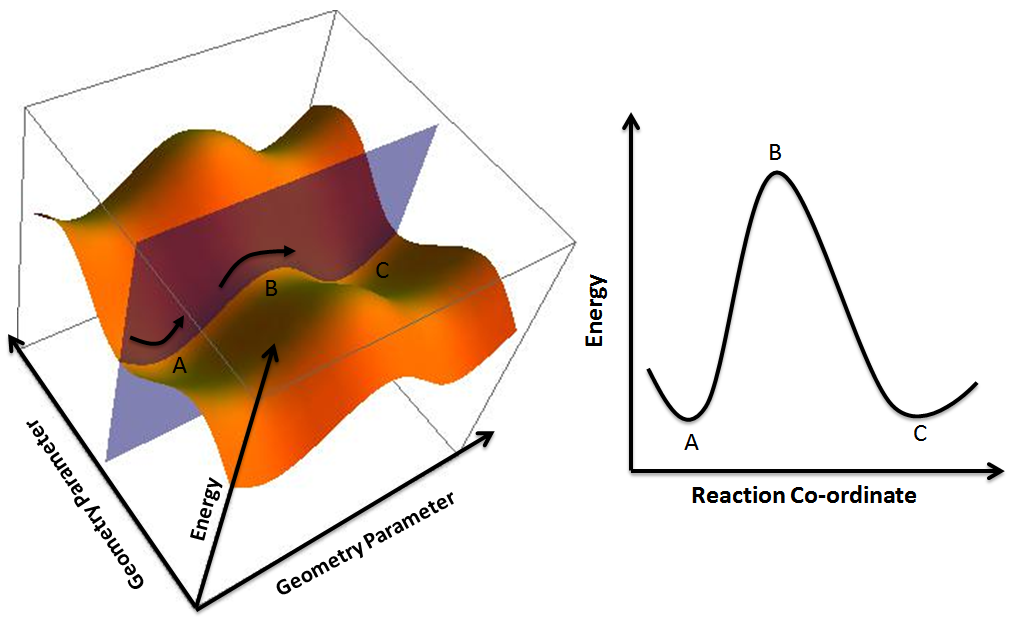
\includegraphics[width=\textwidth]{figures/pes}
  \caption[A typical reaction coordinate diagram.]{A typical reaction coordinate diagram.}
\label{fig:pes}
\end{figure}

In a typical reaction coordinate diagram, the reactants begin to interact and form a pre-reaction complex. Given sufficient energy, the reaction will proceed over the top of the energy barrier through a transition state (TS) complex. After the chemical transformation is completed, a post-reaction complex is formed until the products are able to separate. This is a somewhat simplified description, as it only broadly describes a chemical transformation. In particular, the roles of substrate-radical and substrate-radical-medium interactions along the reaction coordinate are not fully described. This is in fact a key point, as a thorough understanding of these interactions continues to be a hole in the literature.

Consequently, recent work from our group, in collaboration with our experimental colleagues at the University of Rome Tor Vergata, has focused on the importance of substrate-radical interactions in determining the kinetics of HAT reactions. Specifically, it has been shown that the three-dimensional structures of oxygen-centred radicals, as well as the organic substrates, impact the nature of the interactions involved in HAT reaction pathways.\cite{Salamone2015Rev} In our work, we utilize primarily the benzyloxyl (\bno) and cumyloxyl (\cumo) radicals, which serve as a proxy for biological oxygen-centred radicals. This is primarily due to the fact that reactions involving \bno\ and \cumo\ are relatively long lived in solution, and can be monitored using time-resolved laser flash photolysis (LFP) techniques. These radicals are somewhat different than biologically relevant radicals such as \ch{HO^.}, and as a result, the reactivity trends pertaining to the substrates can be somewhat masked by the properties of the radical, such as steric bulk,\cite{Finn2004} or non-covalent binding.\cite{Salamone2011b} Nonetheless, through a careful combination of theoretical and experimental techniques, reactions involving \bno\ and \cumo\ with a variety of organic substrates have been used to develop a great deal of insight with respect to the role of structure in both the radicals and substrates, and resulting intermolecular interactions.

\section{Research goals}

With respect to the work in this thesis, in Chapter~\ref{ch:arrhenius} the importance of the left-hand side of~\ref{fig:pes} shall be examined by studying how the pre-reaction complex impacts HAT reactions. There has been limited investigation of the importance of pre-reaction complex formation for HAT reaction.\cite{Kreilick1966} This is problematic, as oxygen-centred radicals can hydrogen bond with substrates as both acceptors and donors.\cite{Johnson2009a} These hydrogen bonding interactions, in addition to the other non-covalent interactions between the radical and substrate, lead to the formation of a pre-reaction complex. Accordingly, the formation of a pre-reaction complex is a fundamental step in the model systems that have been used to study HAT.

The specific aim of Chapter~\ref{ch:arrhenius} is to investigate the effects of non-covalent binding in the pre-reaction complex, with respect to the well-known, but phenomenological, Arrhenius equation. As of yet, there is no framework which relates the non-covalently bound pre-reaction complex to kinetic results. I ask the simple question: Does there exist a direct correlation between the Arrhenius pre-factor and the non-covalent binding that occurs in the pre-reaction complex formed for HAT reactions? To address this question, I examine the non-covalent binding in the pre-reaction complex in a series of related HAT reactions. Arrhenius parameters for the systems of interest in this work were previously tabulated,\cite{DiLabio2005} and consist of thermoneutral or nearly thermoneutral reactions involving the formation and destruction of oxygen-centred radicals. These reactions are related to the phenol-phenoxyl self-exchange reaction, where a relatively strong pre-reaction complex is expected.

Then in Chapter~\ref{ch:bde}, the right-hand side of~\ref{fig:pes} is considered, where the effects of bond dissociation enthalpies (BDEs) on HAT rate constants are examined. BDEs are central to the understanding of reactions with respect to thermodynamics. In addition to this, there exists a tremendous amount of literature in which BDEs are linked to chemical reactivity, especially for HAT reactions.\cite{Kochi1973, Tedder1982, Wijtmans2003, Pratt2004, Mayer2004} There is a linear free energy relationship (LFER) called the Bell-Evans-Polanyi (BEP) principle,\cite{Bell1936,Evans1938} which states that the difference in activation energy ($E_a$) for two related reactions is proportional to the differences in reaction enthalpy ($\Delta H$):

\begin{equation}
  E_a = E_0 + \alpha \Delta H
  \label{eq:bep}
\end{equation}

\noindent where $E_0$ is the activation energy of a reference reaction, and $\alpha$, a constant which characterizes the position of the TS along the reaction coordinate. This relationship has been more generally used to compare larger families of reactions. Despite the widespread use of the BEP principle, the validity of this relationship is not well described.

I probe the validity of the BEP principle for a series of HAT reaction from \ch{C-H} bonds, with the aim to determine how generally it may be applied. This is achieved by relating accurate, theoretically determined C-H BDEs for species that undergo abstraction at the appropriate C-H position, to the experimentally determined HAT rate constants. HAT reaction rate constants depends on many factors. However, by using rate constants determined under specific conditions (LFP with \cumo\ in acetonitrile at 298K), the differences in reactivity depend mainly on the differences in chemical properties of the substrates of interest. Therefore, I hypothesize that if the BEP relation is valid, there should exist two relationships for C-H bonds: one in which the incipient radical is delocalized into a $\pi$-system (benzylic-allylic), and the other in which the remaining alkyl radicals are largely localized.

Finally, recent experimental results show that non-redox active metal cations, which are found ubiquitously in biological systems, have an inhibitory effect on HAT reactions involving oxygen-centred radicals. This has been demonstrated experimentally for substrates that undergo abstraction from sites adjacent to heteroatoms (e.g.\ amines, amides, and ethers). Under various stoichiometric ratios, these metal cations have effects ranging from full inhibition to partial deactivation of HAT reactivity.\cite{Salamone2013a, Salamone2015metals, Salamone2016} This effect has been attributed partially to the effects of hyperconjugative overlap. Take for example tetrahydrofuran (THF), shown in~\ref{fig:THF}. In the absence of other species, there exists C-H bond weakening hyperconjugative overlap of electron density from one of the oxygen lone pairs and the adjacent C-H $\sigma^*$ anti-bonding orbitals. The interaction of a metal cation with the oxygen lone pairs removes electron density from this interaction, thus increasing the C-H bond strength. As a result, the reactivity of this bond is decreased, as observed from the experimentally-measured 3.2-fold decrease in the rate constant for HAT with \cumo\ in acetonitrile from 6.65 \E{7} \Ms to 7.0 \E{7} \Ms in the presence of 1.0 M \ch{Mg(ClO4)2}.\cite{Salamone2013a}

\begin{scheme}[!htbp]
  \centering
    \begin{overpic}[width=0.65\textwidth]{figures/hyperconjugation.eps}
      \put(-10,75) {\large\textbf{A.}}
    \end{overpic}
    \begin{overpic}[width=0.65\textwidth]{figures/THF.eps}
      \put(-10,75) {\large\textbf{B.}}
    \end{overpic}
  \caption[Hyperconjugative overlap in tetrahydrofuran and the effect of non-redox active metal cations on the transition state complex.]
  {\textbf{A.} Hyperconjugative overlap in tetrahydrofuran. \textbf{B.} The non-redox active metal cation accepts electron density from the heteroatom lone pair, reducing overlap with the C-H $\sigma^*$ anti-bonding orbital, and increasing the C-H bond strength, thus destabilizing the TS complex.}
\label{fig:THF}
\end{scheme}

The nature of the interactions between non-redox active metal cations and organic substrates is poorly understood. This problem is explored in Chapter~\ref{ch:hat}, with the aim to understand the fundamental physico-chemical properties that lead to the observed trends in reactivity. The experimentally observed effects have led us to hypothesize that the presence of non-redox active metal cations has a chemo-protective effect against the radical-induced oxidation of biomaterials such as proteins.

In using theory to study HAT reactions, I hope to contribute to a better understanding of the fundamental properties which govern these reactions, and thus develop insights into the many important biological processes in which HAT takes place.
